\section{Approach}
\begin{frame}{Improving OpenMax}
	\begin{itemize}
		\item Handling negative logits
		      \begin{itemize}
			      \item Value Shift
			      \item Adjust Probabilities
		      \end{itemize}
		\item Introducing weight factors
		      \begin{itemize}
			      \item $ \varphi_N = \frac{1}{N-1}$
			      \item $ \varphi_{\omega} = \frac{1}{\sum_i (1 - \omega_i)}$
		      \end{itemize}
		\item Removing alpha parameter
	\end{itemize}
\end{frame}

\begin{frame}{Research Questions 1}
	\texttt{RQ1}: Can OpenMax performance be enhanced by accounting for negative activation values?
\end{frame}

\begin{frame}{Open-Set Classification Rate}
	Correct Classification Rate (CCR)
	\begin{itemize}
		\item Known samples
		\item Threshold $\theta$
		      \begin{equation}
			      \operatorname{CCR} (\theta) = \frac{| \{ k_{c} | \operatorname{argmax}_{1 \leq n \leq N} y_{c,n} = \tau_{c} \wedge y_{c,n} \geq \theta \}|}{ |K|}
		      \end{equation}
	\end{itemize}
	False Positive Rate (FPR)
	\begin{itemize}
		\item Unknown samples
		\item Threshold $\theta$
		      \begin{equation}
			      \operatorname{FPR}(\theta) = \frac{| \{ u_{c} | \operatorname{argmax}_{1 \leq n \leq N} y_{c,n} \geq \theta \}|}{ |U|}
		      \end{equation}
	\end{itemize}
\end{frame}

\begin{frame}{Defining Scoring System}
	\begin{itemize}
		\item $\Sigma$-Score - Thresholding
		\item $\gamma$-Score $ \gamma = \frac{(\gamma^+ + \gamma^-)}{2}$
		      \begin{equation}
			      \gamma^+ = \frac{1}{|K|} \sum_{c=1}^{|K|} y_{\tau_c}
		      \end{equation}
		      \begin{equation}
			      \gamma^- = \frac{1}{|U|} \sum_{c=1}^{|U|} \left ( 1 - \operatorname{argmax}_{1 \leq n \leq N} y_{c,n} \right)
		      \end{equation}
	\end{itemize}
\end{frame}

\begin{frame}{Baseline ($\gamma$)}
	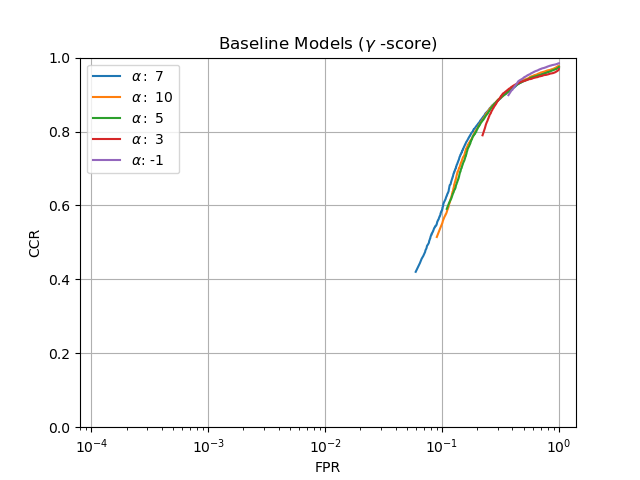
\includegraphics[width=\textwidth]{figures/base_gamma.png}
\end{frame}

\begin{frame}{Baseline ($\Sigma$)}
	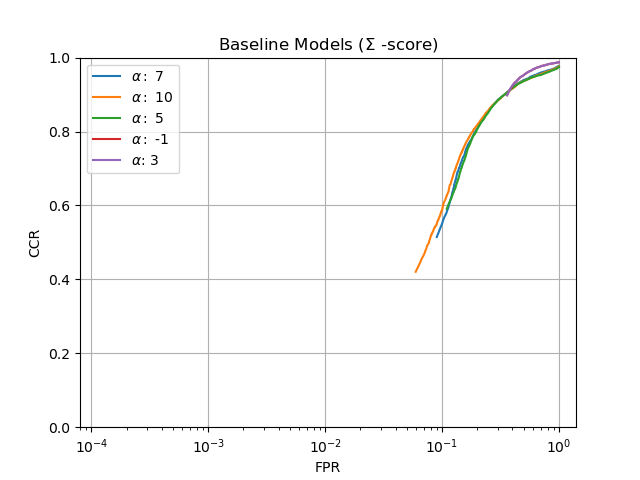
\includegraphics[width=\textwidth]{figures/base_sigma.png}
\end{frame}

\begin{frame}{Results RQ1 ($\gamma$)}
	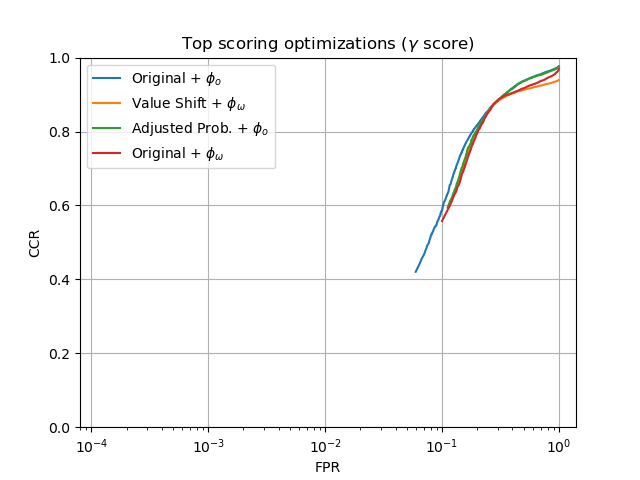
\includegraphics[width=\textwidth]{figures/Top-gamma.png}
\end{frame}

\begin{frame}{Results RQ1 ($\Sigma$)}
	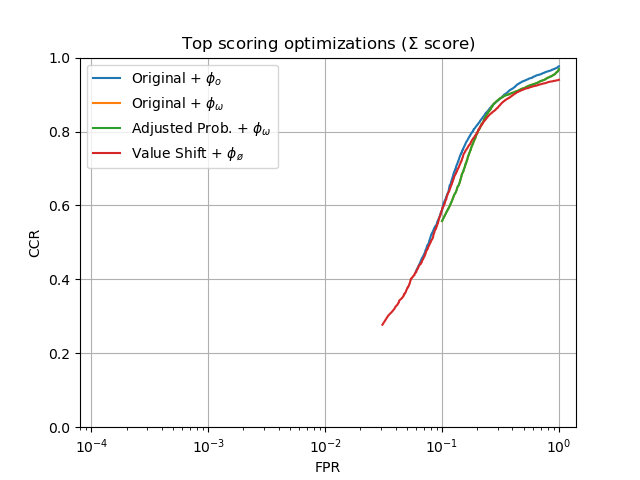
\includegraphics[width=\textwidth]{figures/Top-sigma.png}
\end{frame}

\begin{frame}{Where to apply the clustering?}
	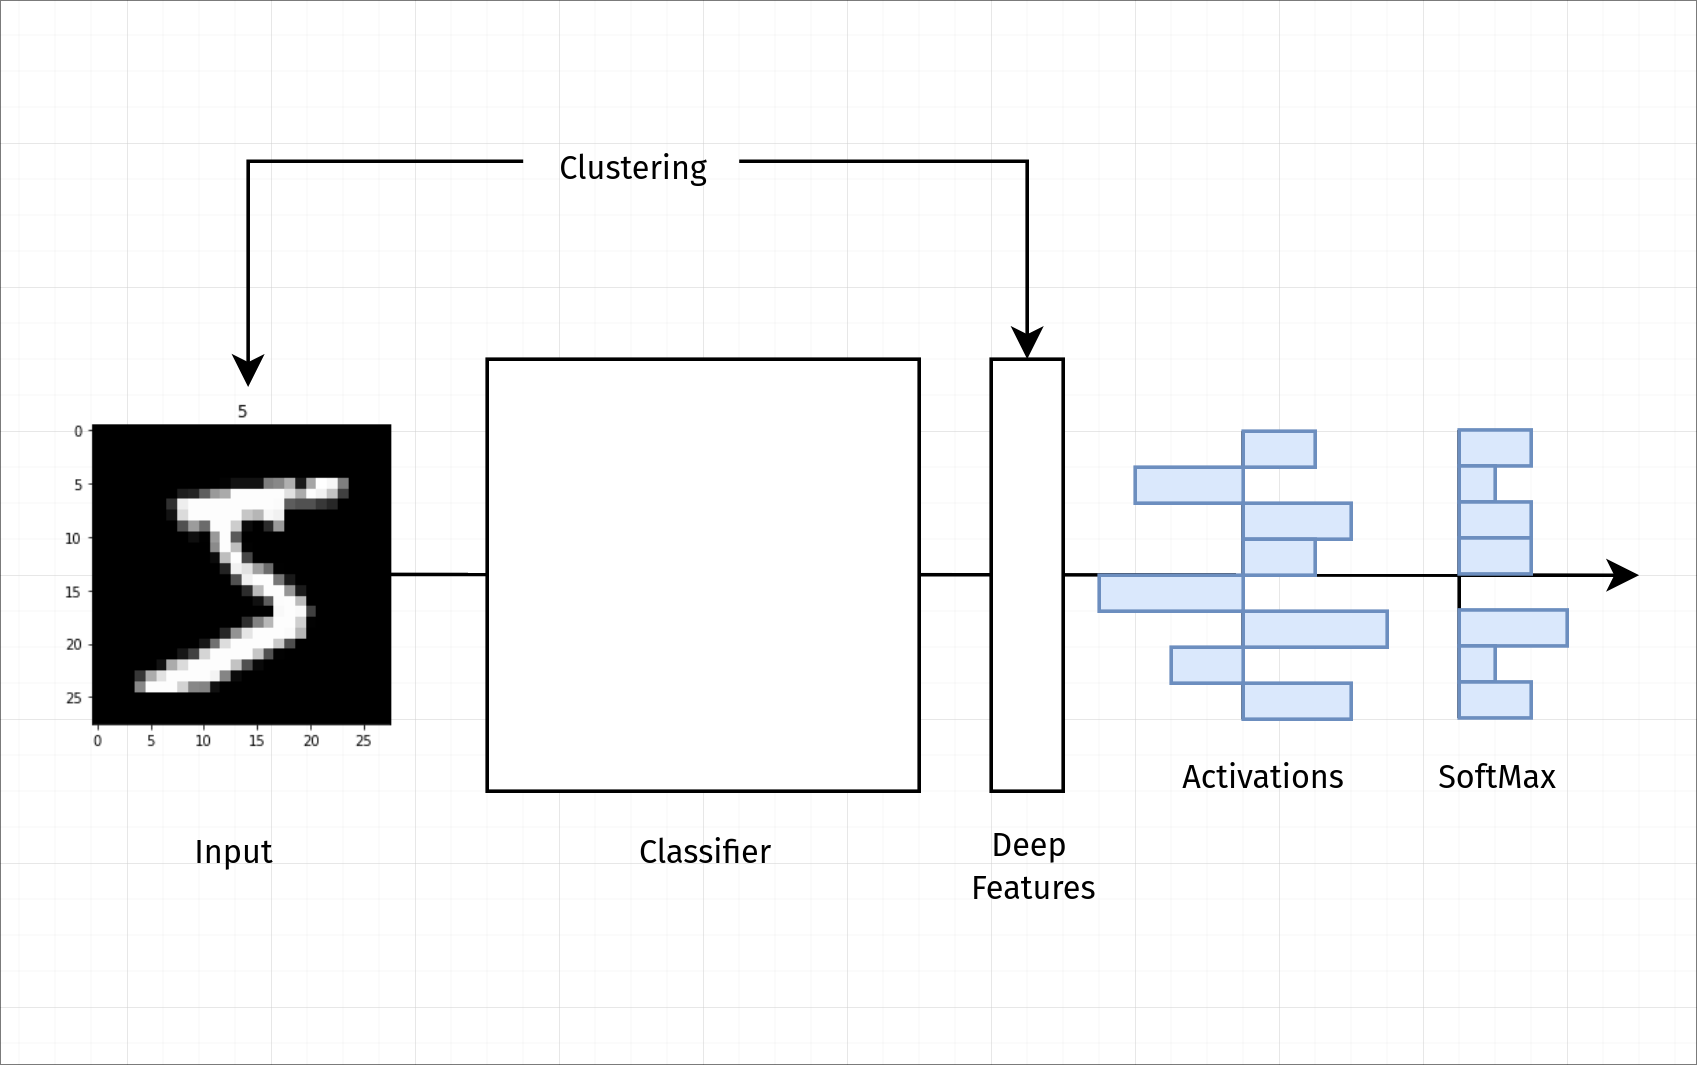
\includegraphics[width=\textwidth]{figures/openmax_clustering.png}
\end{frame}

\begin{frame}{Introducing Clustering to OpenMax}
	Input Clustering:
	\begin{itemize}
		\item Input data
		\item Per class
		\item Each cluster a class
	\end{itemize}
	Features Clustering:
	\begin{itemize}
		\item Training Features
		\item Validation Features
		\item Per class
	\end{itemize}
	Combination of both types
\end{frame}

\begin{frame}{Visualizing Clustering}
	\centering
	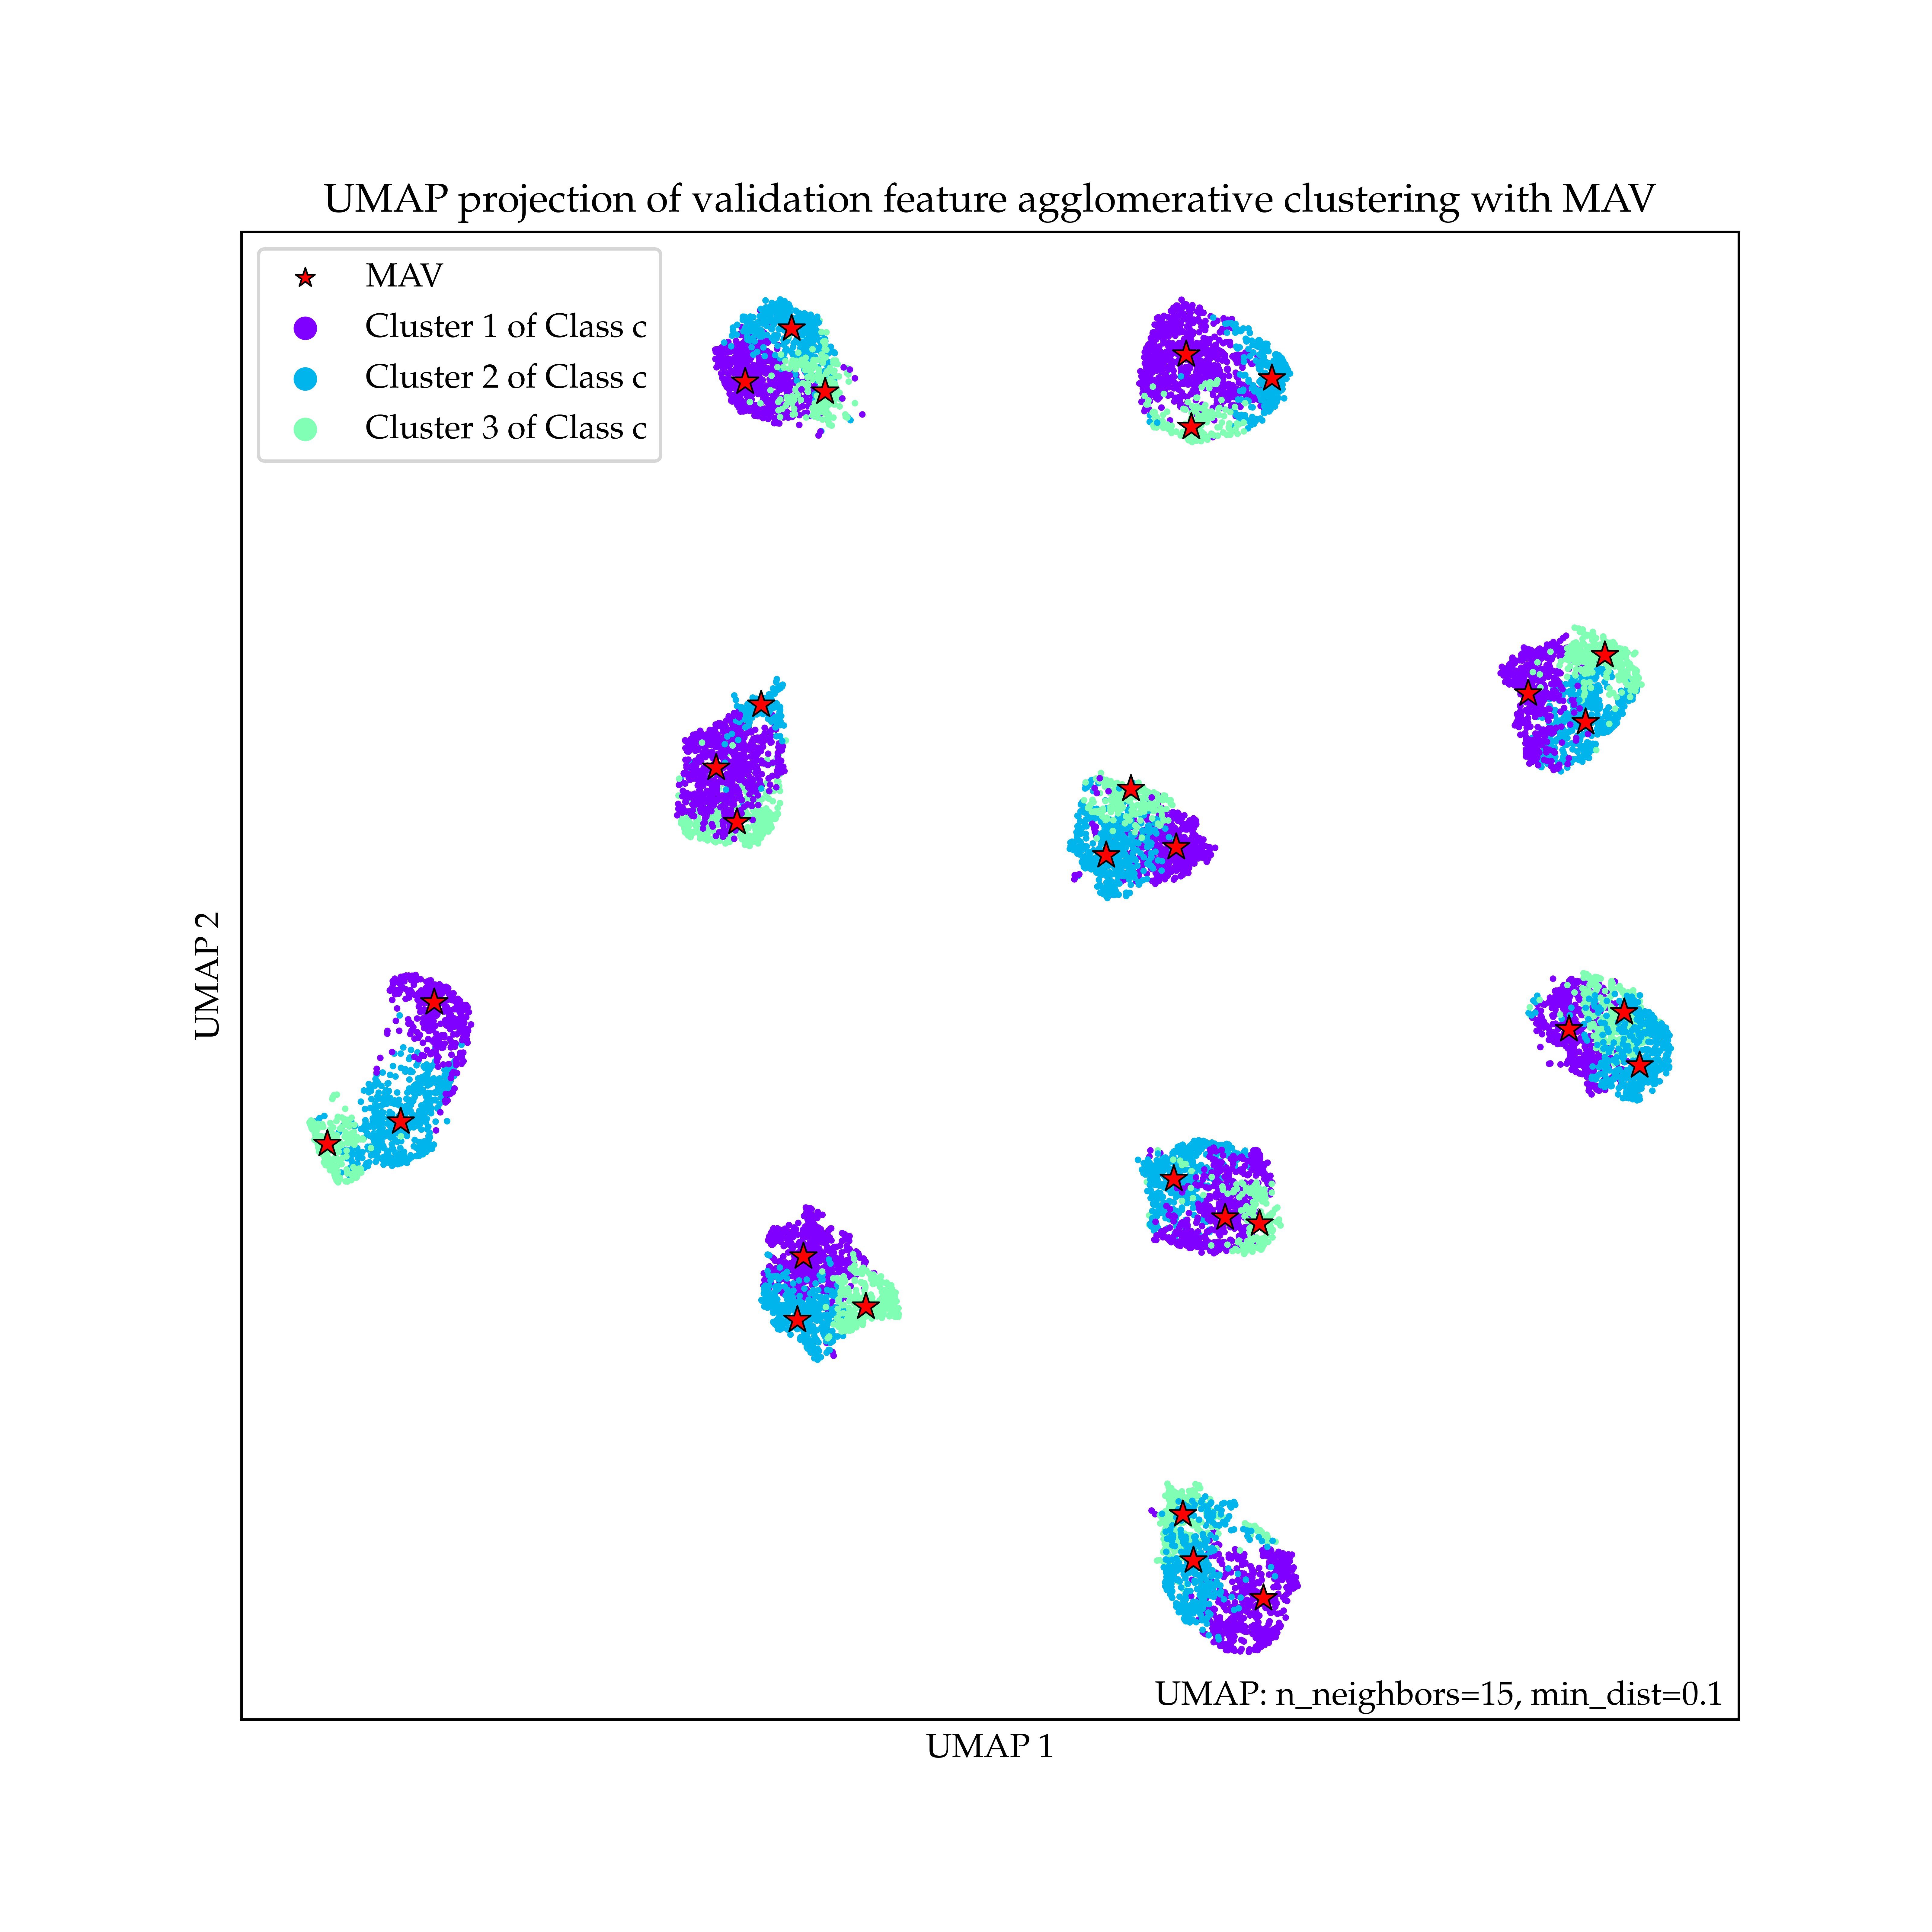
\includegraphics[width=0.75\textwidth]{figures/umap_projection_emnist_cluster.png}
\end{frame}
